\documentclass[capnocolon,titlechinese]{ustcthesis}
\usepackage{coqdoc}
\usepackage{metalogo}
%\usepackage{floatrow}
\usepackage{verbatim}


% 设置图形文件的搜索路径
\graphicspath{{figures/}}
\begin{document}
%%%%%%%%%%%%%%%%%%%%%%%%%%%%%%
%% 封面部分
%%%%%%%%%%%%%%%%%%%%%%%%%%%%%%
  % 中文封面内容
  %如果使用\makeseparatetitle命令生成扉页,当中文标题过长时可以将多余的标题放在\titletail{}中
  \title{分离逻辑的定理证明器的}
  \titletail{设计与实现}
  \entitle{Design and Implementation of Separation Logic Theorem Prover}
  %全角空格可以正常输出
  \author{何春晖}
  \enauthor{He Chunhui}
  \department{计算机科学与技术学院}
  \No{PB09210183}
  \tutor{冯新宇\ 教授}
  \entutor{Prof.Feng Xinyu}
  \cntime{二〇一三年五月}
  \entime{May,2013}
  %生成封面(制本厂要求的格式)
  \makecover
  % 扉页形式
  %生成中英文合并的扉页
  \maketitle
  %生成中英文分开的扉页
  %\makeseparatetitle

%%%%%%%%%%%%%%%%%%%%%%%%%%%%%%
%% 前言部分
%%%%%%%%%%%%%%%%%%%%%%%%%%%%%%
\frontmatter

  % 致谢
  \begin{thankspage}
感谢冯新宇老师、李兆鹏老师和陈意云老师在学习、生活方面对我的帮助、支持和鼓励。冯老师、李老师多次从繁忙工作中抽出时间与我讨论设计方案、传授经验,使我在较短时间内理清了思路,从而顺利完成毕业设计。

感谢与我同行去苏州完成毕业设计的同学,以及苏州的师兄师姐们。近三个月的学习生活令人难忘。

感谢父母。
\end{thankspage}

  % 目录

  \tableofcontents
  % 摘要
  \begin{cnabstract}
本文针对程序验证中定理自动证明的需求,从头实现了一个分离逻辑的定理证明器。相比Z3等自动证明系统,本文实现的证明器能够验证分离逻辑的定理,并且能够输出Coq兼容的证明项;而相比Coq等交互式证明系统,则具有完全自动化、验证速度快的优势。从而在定理证明器的表达能力、自动化和可信性三方面达到了较好的平衡。

\cnkeywords{程序验证,自动定理证明,分离逻辑,Coq兼容证明项生成}
\end{cnabstract}

\begin{abstract}
We implement a separation logic theorem prover for program verification from scratch.
\keywords{Program Verification, Automatic Theorem Prover, Separation Logic, Coq-Compatible Proof Term Generation}
\end{abstract}



%%%%%%%%%%%%%%%%%%%%%%%%%%%%%%
%% 正文部分
%%%%%%%%%%%%%%%%%%%%%%%%%%%%%%
\mainmatter
  \chapter{绪论}
\label{chap:intro}

\section{研究背景}
\subsection{程序验证}
\subsection{分离逻辑}
\subsection{自动定理证明器}
\subsection{}
\section{相关工作}
\section{}
  %绪论
  \chapter{证明器的总体设计}
\label{chap:struct}
本章给出证明器的总体设计,并说明证明器的各个部分之间如何协作证明一个命题。

\section{输入语言}
本文设计的证明器需要证明的命题可以分成两部分:一部分是纯的一阶逻辑及其理论,另一部分是分离逻辑。前者主要表达程序中变量、函数之间的相等和不等关系,后者主要表示程序中数据结构的变化。

两者在各自推理的同时,前者也为后者服务,如向后者提供指针运算、指针相等关系等内容。这决定了证明器要支持一阶逻辑中的算术理论和相等理论。

由上述需求,我们设计的命题语言如图\ref{struct:syntax}所示。

\begin{figure}[!htbp]
  \centering
  \begin{tabular}{rrcl}
    整数常元 & $C$ & \sep & $0$ \deli{} $1$ \deli{} $-1$ \deli{} \ldots \\
    整型变元 & $X$ & \sep & $x_0$ \deli{} $x_1$ \deli{} $x_2$ \deli{} \ldots \\
    未解释函数 & $F$ & \sep & $f_0$ \deli{} $f_1$ \deli{} $f_2$ \deli{} \ldots \\
    命题变元 & $A$ & \sep & $A_0$ \deli{} $A_1$ \deli{} $A_2$ \deli{} \ldots \\
    公式项  & $T$ & \sep & $C$ \deli{} $X$ \deli{} $F(T,$\ldots$,T)$ \deli{} $+(T, T)$ \deli{} $\cdot(C,T)$ \\
    一阶逻辑原子公式 & $Y$ & \sep{} & $T \le T$ \deli{} $T = T$ \deli{} $A$ \deli{} $\mathrm{true}$ \\
    一阶逻辑公式 & $\Pi$ & \sep{} & $Y$ \deli{}  $\lnot \Pi$ \deli{} $\Pi \impl \Pi$ \deli{} $\Pi \land \Pi$ \deli{} $\Pi \lor \Pi$ \\
    分离逻辑原子公式 & $H$ & \sep{} & $T \mapsto T$ \deli{} $\mathrm{emp}$ \\
    分离逻辑公式 & $\Sigma$ & \sep{} & $H$ \deli{} $\Sigma \ast \Sigma$ \\
    命题 & $P$ & \sep & $ \Pi \land \Sigma \impl \Pi' \land \Sigma' $
  \end{tabular}
  \caption{命题语言的语法}
  \label{struct:syntax}
\end{figure}

证明器接受的命题的整体是一个蕴含式,前件和后件都分别由$\Pi$和$\Sigma$两部分构成,分别代表一阶逻辑部分和分离逻辑部分。

$\Pi$和$\Pi'$是一个无量词的一阶逻辑公式。二元函数$+$和$\cdot$分别解释为整数环上的加法和数乘运算,这意味着只能支持线性的整数算术;除此之外,可出现有限个有限元的函数,它们是未解释的。

$\Sigma$和$\Sigma'$是包含分离逻辑符号的公式。为简化起见,分离逻辑公式只能用$\ast$(分离合取)联结词连接,原子公式只能是$\mathrm{emp}$和$T_1 \mapsto T_2$的形式,分别代表空堆和仅包含一项的堆。

命题语言语义的定义如图\ref{struct:semantic}。
\begin{figure}[!htbp]
  \centering
  \begin{tabular}{rcl}
    $s, h \models P$ & & \\
    $s$是栈 & & $s: T \impl \mathbb{Z}$ \\
    $h$是堆 & & $h: \mathbb{Z} 	\backslash \{0\} \rightharpoonup \mathbb{Z}$ \\
    $s, h \models t_1 = t_2$ & $\iff$ & $s(t_1) = s(t_2)$ \\
    $s, h \models t_1 \leq t_2$ & $\iff$ & $s(t_1) \leq s(t_2)$ \\
    $s, h \models \mathrm{true}$ & $\iff$ & 真 \\
    $s, h \models \lnot P$ & $\iff$ & $s, h \models P$为假 \\
    $s, h \models P \impl Q$ & $\iff$ & 若$s, h \models P$,则$s, h \models Q$ \\
    $s, h \models P \land Q$ & $\iff$ & $s, h \models P$ 且 $s, h \models Q$ \\
    $s, h \models P \lor Q$ & $\iff$ & $s, h \models P$ 或 $s, h \models Q$ \\
    $s, h \models \mathrm{emp}$ & $\iff$ & $\mathrm{dom}(h)= \emptyset$ \\
    $s, h \models t_1 \mapsto t_2$ & $\iff$ & $s(t_1) \neq 0$ 且 $\mathrm{dom}(h) = \{s(t_1)\}$ \\
    & & 且 $h(s(t_1)) = s(t_2)$ \\
    $s, h \models P \ast Q$ & $\iff$ & 存在$h1, h2$, $h1 \bot h2$ 且 $h = h1 \ast h2$ \\
    & & 且 $s, h1 \models P$ 且 $s, h2 \models Q$ \\
  \end{tabular}
  \caption{命题语言的语义}
  \label{struct:semantic}
\end{figure}

由于分离逻辑隐式包含了堆,这在纯的一阶逻辑中是没有的。因此图中的语义定义主要说明了一阶逻辑符号拓展到有堆出现时的意义。

\section{证明项}
证明项是一种语言,它可以用来表示证明的推理过程。本文实现的证明器通过对每一个命题出具Coq兼容的证明项,来满足携带证明代码对携带机器可检查证明的要求。

\subsection{相关概念}
\subsubsection{Curry-Howard同构}
Curry-Howard同构\cite{HowardWA:fortnc}是指逻辑演算系统与程序类型系统的相对应关系。它指出,自然推理系统与$\lambda$-演算的对应关系如表\ref{tab:curry}。
\begin{table}[!ht]
  \label{tab:curry}
  \caption{自然推理系统与$\lambda$-演算的对应关系}
  \centering
  \begin{tabular}{cc}
    \whline
    自然推理 & $\lambda$-演算 \\
    \hline
    假设 & 对应类型的自由变量 \\
    蕴含引入 & 函数抽象 \\
    蕴含消去 & 函数应用 \\
    定理 & 对应类型的表达式 \\
    \whline
  \end{tabular}
\end{table}

于是,命题的证明问题就可以看作一个寻找对应类型的$\lambda$-表达式的过程。
例如,我们欲证明希尔伯特系统中的L1:
$$ \vdash P \impl (Q \impl P) $$

我们可以构造如下$\lambda$-表达式:
$$\lambda (H_0: P).(\lambda (H_1: Q).H_0)$$

上式的类型为$P \impl (Q \impl P) $,因此它是L1的一个证明。

\subsubsection{归纳构造演算与Coq}
归纳构造演算(Calculus of Inductive Constructions)是一种$\lambda$-演算的扩展,它结合了逻辑中的一些最新进展,因而能力更强。

Coq\cite{coq}是一个基于归纳构造演算的高阶逻辑定理证明辅助系统。其独到之处在于,表达程序和表达证明都使用同一套语言。

上一节L1的证明用Coq证明项表达如下:
\begin{verbatim}
    (fun H0:P => (fun H1:Q => H0))
\end{verbatim}

\subsection{表达证明项的数据结构}
我们将证明项保存为一个类似$\lambda$-表达式的形式。

证明项类型叫做\texttt{proof},定义用类ML语言描述如下:
\begin{verbatim}
    type param = (string * prop)        (* 参数 *)
    type proof =
    | Hole                               (* 空 *)
    | Id of string      (* 公理、定理、变量标识 *)
    | Lam of param list * proof    (* 函数抽象 *)
    | App of proof list            (* 函数应用 *)
\end{verbatim}

\texttt{Lam}和\texttt{App}构造分别模拟$\lambda$-表达式的函数抽象和函数应用。唯一不同的是,参数部分都被扩展成了列表,以更加便于实际使用。

\texttt{Hole}代表空,意味着没有找到命题的证明。

\texttt{proof}并不能表达纳构造演算的所有构造,但是在本文设计的证明器是足够用的。

\section{结构及流程}

\begin{figure}[!htbp]
  \centering
  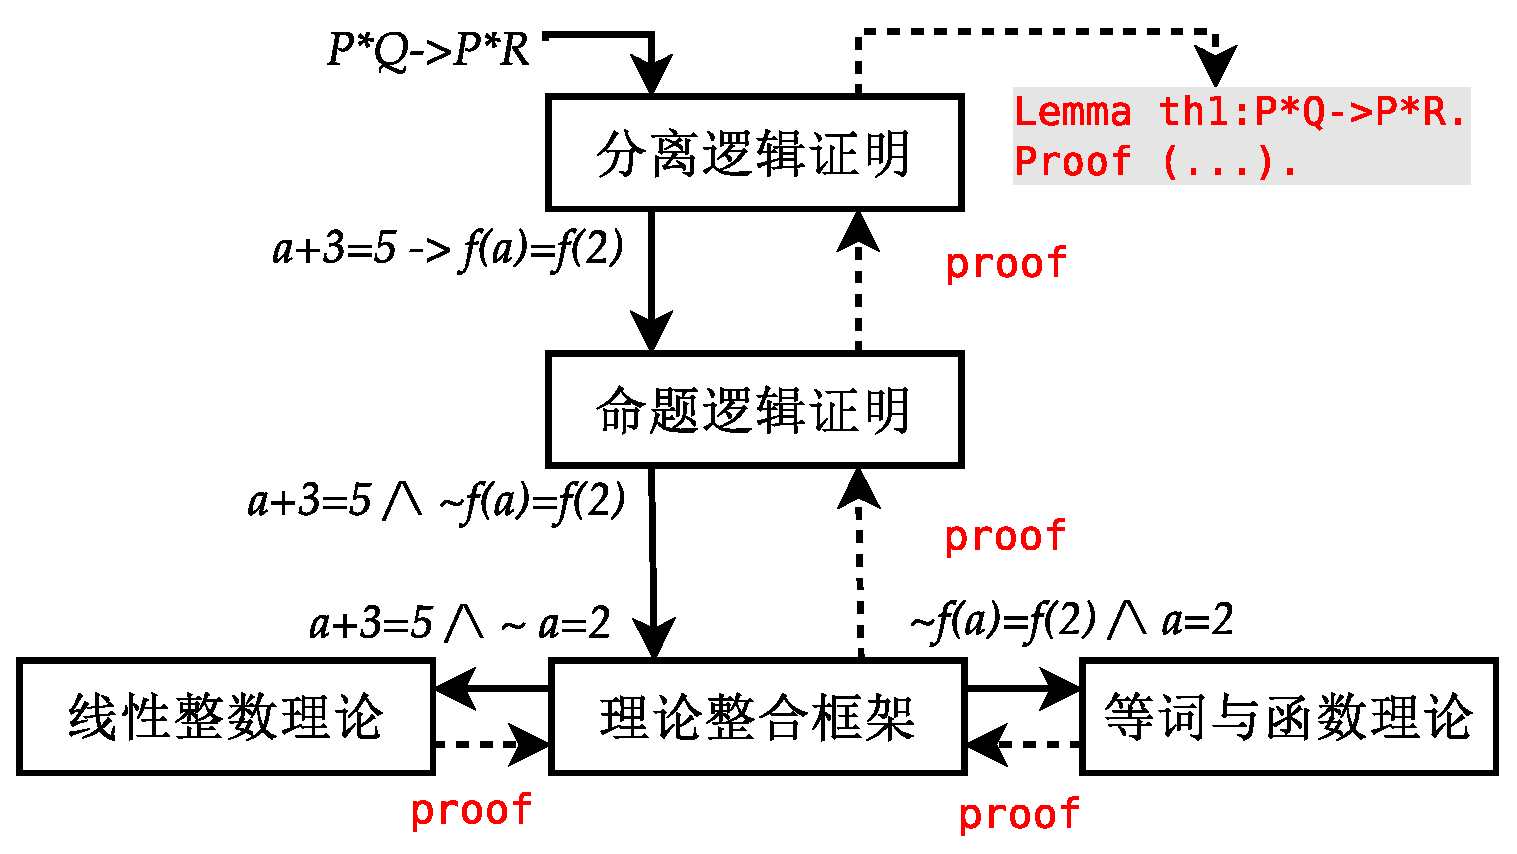
\includegraphics[width=0.8\textwidth]{stru.eps}
  \caption{证明器的结构}
  \label{struct:fig}
\end{figure}

如图\ref{struct:fig}所示,证明器逻辑上可以分成两大部分。一部分是传统的基于一阶逻辑的证明器;另一个部分是分离逻辑的证明器。

\subsection{分离逻辑的证明器所做的工作}
证明器开始运行时,接收命题语言$\Pi \land \Sigma \impl \Pi' \land \Sigma'$。

这个命题的证明可以化为求证:
\begin{eqnarray}
  \vdash & \Pi \land \Pi'' \impl \Pi' \label{struct:eq1}\\
  \vdash & \Pi \land \Sigma \impl \Sigma' \label{struct:eq2}
\end{eqnarray}

\ref{struct:eq1}式是一个纯的一阶逻辑的证明过程,因此直接将该部分命题发送到一阶逻辑的证明器求证。其中$\Pi''$是分离逻辑部分中推出的一些算术信息,如指针非空和不同堆的地址不同。

\ref{struct:eq2}式是一个带分离逻辑的证明过程。该部分将由分离逻辑的证明器使用分离逻辑中的定理将该过程分解成求证一系列纯一阶逻辑命题,并发送到一阶逻辑的证明器求证。该部分的方法在第\ref{chap:sep}章说明。

分离逻辑的证明器综合两式,得到命题的最终证明。

\subsection{一阶逻辑的证明器所做的工作}
一阶逻辑的证明器结构属于目前较先进的SMT(Satisfiability Modulo Theories)证明器结构。

对于每一个被发送到一阶逻辑的证明器的命题,首先经过命题逻辑证明模块。该模块将所有不同的公式项看作一个独立的命题变元,最终化简成为约束满足(SAT)问题,该步的具体方法在第\ref{chap:sat}章说明。

由于命题逻辑证明求解时不会关心命题公式项的具体内容,因此它在求解时会生成一系列可能否证命题的``反例''赋值。这些``反例''重新构成命题后被发送到理论整合框架。在这个框架中,命题被按照公式项分成不同的部分,送给不同的理论求解器求解。由于考察公式项的具体结构,``反例''将被一一反驳。该步具体方法在第\ref{chap:euf}、\ref{chap:lia}、\ref{chap:no}章说明。

命题逻辑证明模块综合这些反驳信息,得到一阶逻辑命题的最终证明。
 %证明器的总体设计
  \chapter{Coq证明项的构造概述}
\label{chap:proof}

\section{Coq}
\section{证明项的数据结构}
\section{证明项构造的主要方法}
  %Coq证明项的构造概述
  \chapter{命题逻辑命题的证明}
\label{chap:sat}

\section{输入语言}
\begin{figure}[!htbp]
  \centering
  \begin{tabular}[rcl]{rcl}
    & & $Y$是原子公式 \\
    $\Pi$ & \sep{} & $Y$ \deli{} $\lnot \Pi$ \deli{} $\Pi \impl \Pi$ \deli{} $\Pi \land \Pi$ \deli{} $\Pi \lor \Pi$ \\
  \end{tabular}
  \caption{命题逻辑语言}
  \label{sat:syntax}
\end{figure}
本部分接收的语言是纯一阶逻辑命题的\emph{命题框架}。命题框架是指,不理会原子公式的具体结构,只是简单地将不同的原子公式看作不同的命题变元。

\section{结构}
\begin{figure}[!htbp]
  \centering
  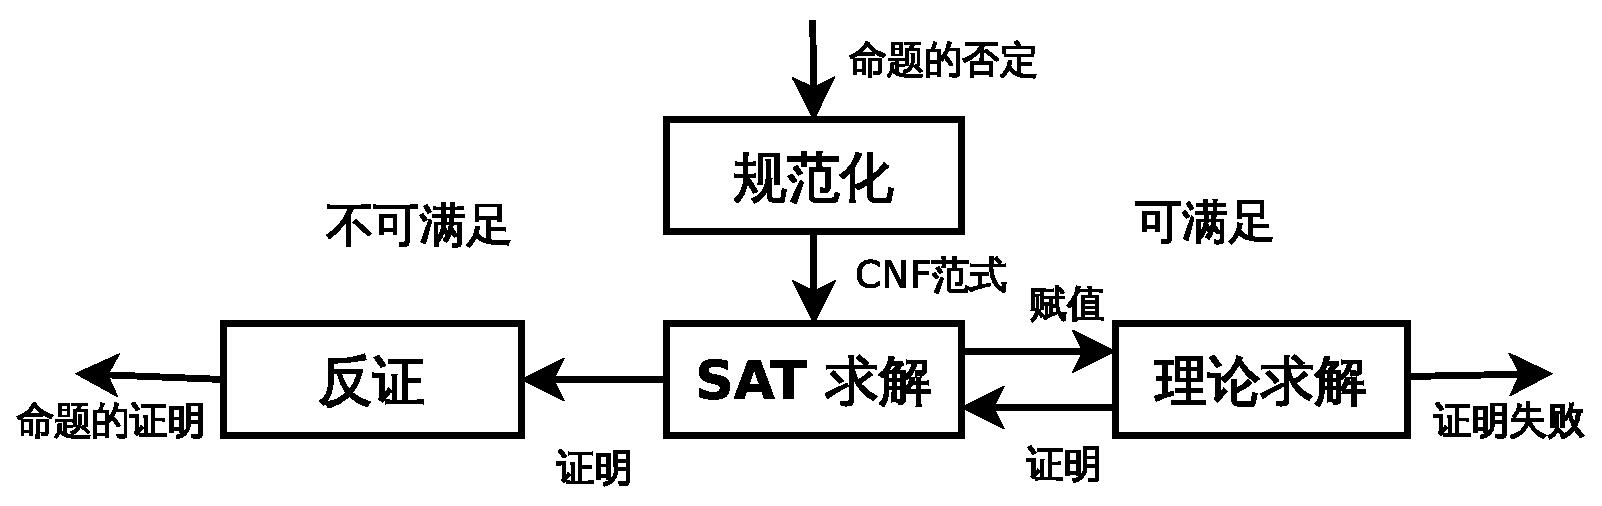
\includegraphics[width=0.8\textwidth]{sat-stru.eps}
  \caption{命题逻辑证明的结构}
  \label{sat:stru}
\end{figure}
如图\ref{sat:stru},本部分的核心是一个SAT求解器。

SAT求解器能够解决下列一类问题:

\begin{definition}[SAT问题]
设X是布尔变量集,$|X|=n$,$\alpha$是合取范式,并有$\alpha = \bigwedge_i (\bigvee_{j_1} x_{ij_1} \lor \bigvee_{j_2} \lnot x_{ij_2})$,$x_{ij} \in X$。

求一种赋值方法$(b_1, b_2, \dots, b_n)$,使得$\alpha$为真。若不存在这种赋值方法,则称$\alpha$不可满足。
\end{definition}

我们使用下面的定理来利用SAT求解器证明定理:

\begin{theorem}
  若$\lnot \alpha$不可满足,则$\vdash \lnot \lnot \alpha$。
\end{theorem}

待证的命题首先被否定并化为合取范式(CNF)$\alpha'$,然后送往SAT求解器求解。SAT求解器有可能返回两种结果:可满足和不可满足。

若结果为不可满足,如图\ref{sat:stru}左半部分,则说明$\vdash \lnot \lnot \alpha$,直接将SAT求解过程的证明证明项取出,并应用在Coq定义的双重否定引理:
\begin{verbatim}
  Lemma NNPP : forall p:Prop, ~ ~ p -> p.
\end{verbatim}
即可得证。

若结果为可满足,如图\ref{sat:stru}右半部分,将得到一个原子命题的赋值向量$\vec{v}=(b_1, b_2, \dots , b_n)$。这说明,单从命题的命题框架看,无法得出命题在赋值$\vec{v}$下成假。

此时,利用命题编码,可以将赋值转换成一个原子命题的合取形式:
\begin{definition}[命题编码]命题编码是指合取式
  $$\beta = \bigwedge_i y_i$$
  其中
  \begin{equation*}
    y_i =
    \begin{cases}
      x_i & \text{若}x_i = b_i = \mathrm{true} \\
      \lnot x_i & \text{若}x_i = b_i = \mathrm{false}
    \end{cases}
  \end{equation*}
  $$ x_i \in X $$
\end{definition}


此时将此编码$\beta$送到理论求解器求解。理论求解器若能得出成假结论,则重新触发SAT求解器继续求解;否则,证明失败。

\section{SAT求解}
\subsection{DPLL算法}
本文实现的SAT求解器使用DPLL算法求解。

DPLL算法是由Davis、Putnam、Loveland、Longemann联合提出的一种求解SAT问题的完备方法。

DPLL算法的核心是回溯法。如图\ref{sat:dpll}求解的是合取范式$P \land (\lnot P \lor Q) \land \lnot Q$的可满足赋值的搜索树。

\begin{figure}[!htbp]
  \centering
  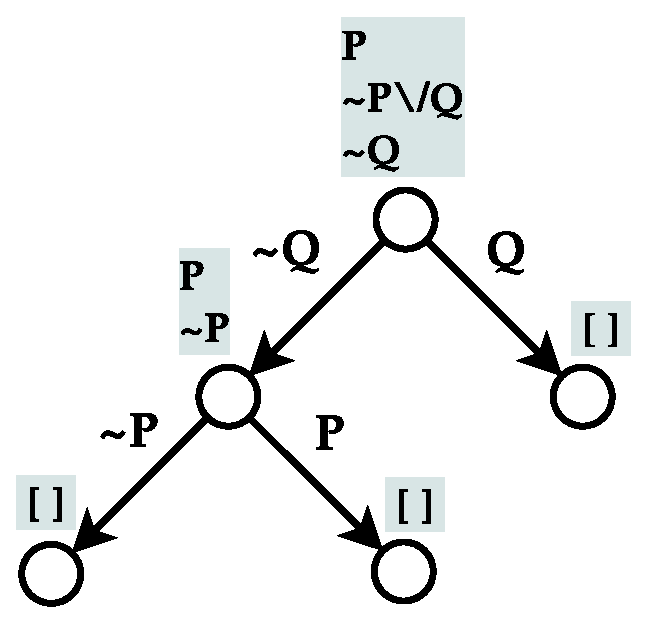
\includegraphics[width=0.35\textwidth]{sat.eps}
  \caption{DPLL算法的的搜索树}
  \label{sat:dpll}
\end{figure}

算法首先尝试$Q$的赋值。当$Q$赋值为真,则与范式中的$\lnot Q$矛盾,因此不可行,回溯;当$Q$赋值为假时,原式变为$P \land (\lnot P \lor \mathrm{false}) \land \mathrm{true}$,即$P \land \lnot P$,然后对$P$做相同的尝试,直到找到一个赋值使得命题成真。

本例经过尝试,发现没有成真的赋值,返回不可满足。

DPLL算法还有不少优化:
\begin{enumerate}
  \item 变量删减:将式子中仅出现正文字或仅出现反文字的变量删除
  \item 变量排序:按照一定的次序搜索,加快剪枝
  \item 约束传播:尽早由部分赋值发现矛盾
  \item 常数时间回溯等
\end{enumerate}
在这些优化下,DPLL算法能够求解变量数上千的SAT问题。

\subsection{证明项的构造}
DPLL算法的证明项构造一般基于归结(resolution)规则构造:
$$\vdash (P \lor Q) \land (\lnot P \lor R) \impl Q \lor R$$
其中$P$、$Q$、$R$都是一阶公式。

当使用归结规则构造DPLL算法的证明项时,需要先对搜索树做若干分析,才能生成证明项,不是很直接。本文提出一个直接生成证明项的方法。

简单地说,这个方法基于如下定理:
$$\alpha' \land E \vdash (P \impl \mathrm{false}) \impl (\lnot P \impl \mathrm{false}) \impl \mathrm{false} $$
其中$\alpha'$是合取范式,$E$是部分赋值的命题编码,$P$是范式中的某一文字。

其意义为:在部分赋值$E$下,若文字$P$赋值为真,最终得到矛盾,且文字$P$赋值为假,最终也得到矛盾,则$\alpha'$不可满足。

应用时,只需要在DPLL搜索树的每个节点按照后序遍历使用即可生成证明。以图\ref{sat:dpll}为例,其生成的证明序列是:
\begin{align*}
  P \land (\lnot P \lor Q) \land \lnot Q \land Q \land P & \vdash \mathrm{false} & (1) & \quad P \land (\lnot P \lor Q) \land \lnot Q \\
  P \land (\lnot P \lor Q) \land \lnot Q \land Q \land \lnot P & \vdash \mathrm{false} & (2) & \quad P \land \lnot P \\
  P \land (\lnot P \lor Q) \land Q \land Q  & \vdash \mathrm{false} & (3) & \quad \text{由定理及(1) (2)}\\
  P \land (\lnot P \lor Q) \land Q \land \lnot Q & \vdash \mathrm{false} & (4) & \quad Q \land \lnot Q \\
  P \land (\lnot P \lor Q) \land Q & \vdash \mathrm{false} & (5) & \quad \text{由定理及(3) (4)}
\end{align*}

\section{命题的规范化}
命题规范化要做的事是将任意的命题化成SAT求解器能够求解的合取范式的形式。

化简过程分为两步:先将命题化简为否定范式(NNF),再将否定范式化为合取范式。

\subsection{规范到否定范式}
规范到否定范式一共要做两件事:消除蕴含词$\impl$;将否定词$\lnot$深入到文字上,并且保证文字前最多只有一个否定词。

从语法结构的观点看,本步骤实际上是由一棵语法树变换到另一棵语法树。由于语法树是由图\ref{sat:syntax}构造地定义的,因此只需要考察每一个局部结构的变化情况,再逐级递归即可。

\subsubsection{变换分类}
变换一共分两种情形:A型、B型。图中虚线代表递归时应该看作整体。
\begin{figure}[!h]
\centering
\subfigure[and]{
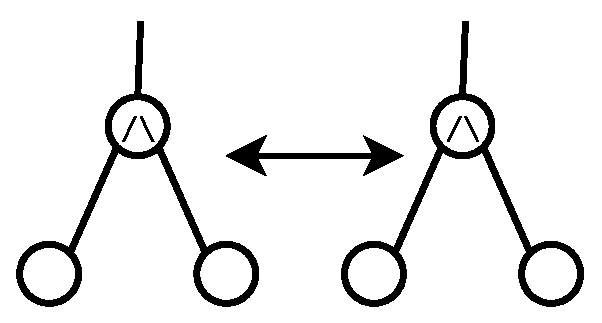
\includegraphics[width=0.27\textwidth]{nnf-and.eps}}
\subfigure[or]{
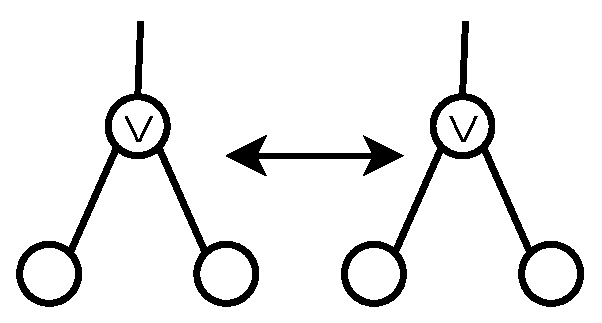
\includegraphics[width=0.27\textwidth]{nnf-or.eps}}
\subfigure[not Y]{
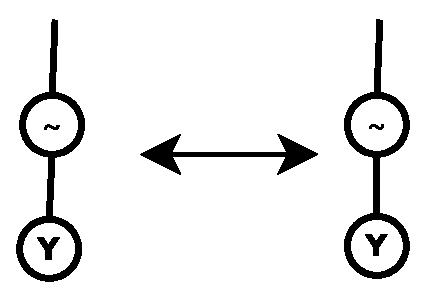
\includegraphics[width=0.19\textwidth]{nnf-np.eps}}
\subfigure[Y]{
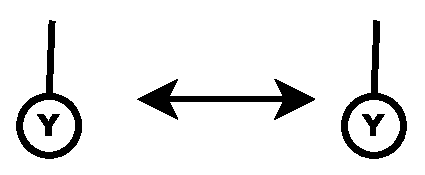
\includegraphics[width=0.19\textwidth]{nnf-p.eps}}
\caption{A型:结构不变}
\end{figure}

\begin{figure}[!h]
\centering
\subfigure[not and]{
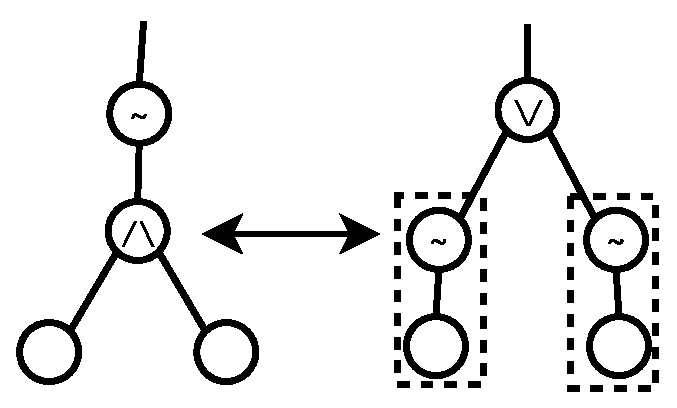
\includegraphics[width=0.32\textwidth]{nnf-nand.eps}}
\subfigure[not or]{
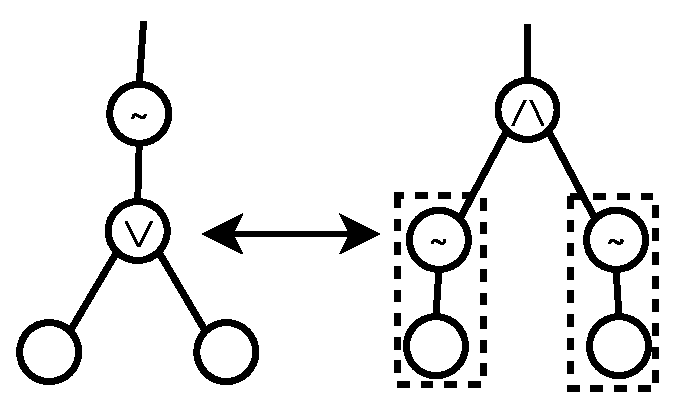
\includegraphics[width=0.32\textwidth]{nnf-nor.eps}}
\subfigure[not not Y]{
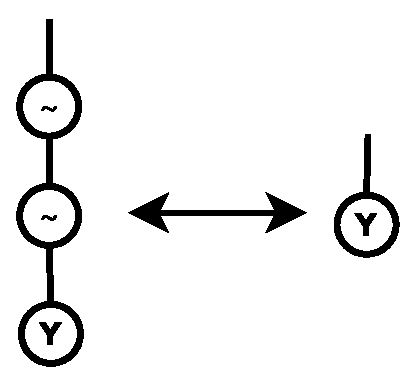
\includegraphics[width=0.19\textwidth]{nnf-nnp.eps}}
\subfigure[imply]{
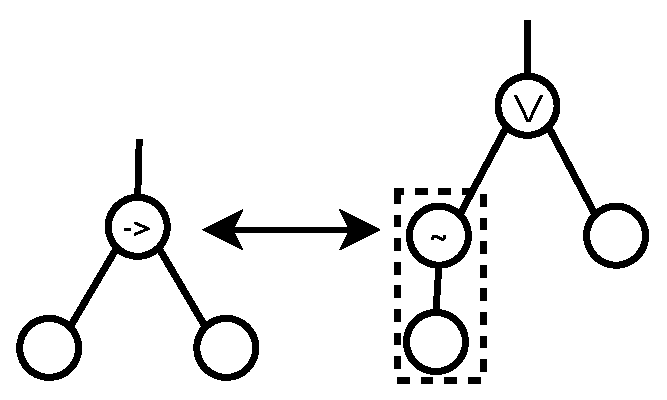
\includegraphics[width=0.32\textwidth]{nnf-imp.eps}}
\subfigure[not imply]{
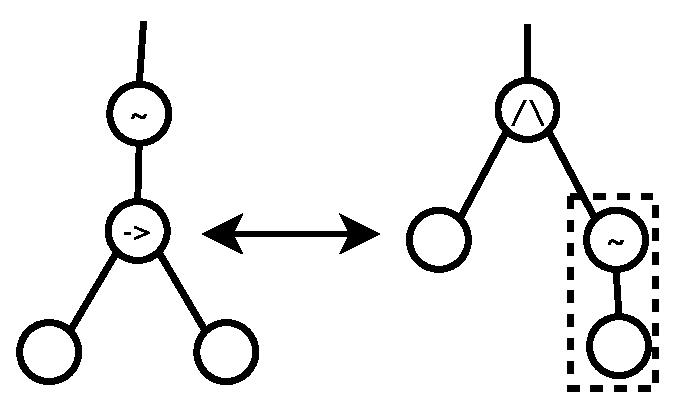
\includegraphics[width=0.32\textwidth]{nnf-nimp.eps}}
\caption{B型:结构改变}
\end{figure}

\subsubsection{证明项构造}
证明项的构造是直接的,只需在递归时引用Coq中预定义的引理即可。

每一种情况对应一个引理,罗列如下。

\paragraph{A型引理}
\begin{verbatim}
Lemma L_and: forall A B C D:Prop, (A<->B)->(C<->D)->((A/\C)<->(B/\D)).
Lemma L_or: forall A B C D:Prop, (A<->B)->(C<->D)->((A\/C)<->(B\/D)).
Lemma L_not: forall A B:Prop, (A<->B)->((~A)<->(~B)).
Lemma iff_p: forall P:Prop, P<->P.
\end{verbatim}

\paragraph{B型引理}
\begin{verbatim}
Lemma iff_nand: forall P Q:Prop, ~(P/\Q) <-> (~P\/~Q).
Lemma iff_nor: forall P Q:Prop, ~(P\/Q) <-> (~P/\~Q).
Lemma iff_nnp: forall P:Prop, ~~P<->P.
Lemma iff_imp: forall P Q:Prop, (P->Q)<->(~P\/Q).
Lemma iff_nimp: forall P Q:Prop, ~(P->Q)<->(P/\~Q).
\end{verbatim}

\subsection{规范到合取范式}
\subsubsection{变换}
从否定范式规范到合取范式是简单的,只需要递归地对公式中的$\lor$做对$\land$的分配律即可。

\subsubsection{证明项构造}
理论上,只要在变换时引用$\lor$对$\land$的分配引理,即可得到合取范式的证明项。但是实践上这样会存在$\land$和$\lor$上交换律和结合律的问题。

例如,$P \lor (Q \lor R)$和$(P \lor Q) \lor R$在日常的非严格的推理中,是看作相同的。但是在Coq系统中却是两个完全不同的类型。若要是类型相等,必须引用结合律。

因此,直接采用分配律后构造证明项后,结果的语法树几乎一定会出现很多“枝杈”,而非规范的右结合树。不是规范形式将会给SAT求解器的证明项构造带来很大负担。

本文提出一个直接由否定范式树生成合取范式每一个的合取支规范形式的方法。

下面以$P \lor (Q \land R)$为例,说明其基本步骤。

\paragraph{从合取范式树抽取合取支}
上式的合取范式为$(P \lor Q) \land (P \lor R)$。容易编写一个递归的过程,抽取出合取支$(P \lor Q)$和$(P \lor R)$并暂存。

\paragraph{决定规范形式}
这里可以根据需要(如根据SAT求解器的内部表示)决定每一个合取支的规范形式,如取为$P \lor Q$和$R \lor P$。

\paragraph{生成合取支的一个析取成分的证明项}
选择$P \lor Q$和$R \lor P$里面一个较好证明的析取支,这里都选择$P$。
即证明:
$$ \vdash P \lor (Q \land R) \impl P $$

由于前件是否定范式,很容易根据$\land$和$\lor$的结构,写一个递归过程,引用Coq如下定理得到证明:
\begin{verbatim}
Lemma and_ind : forall A B P : Prop, (A -> B -> P) -> A /\ B -> P.
Lemma or_ind : forall A B P : Prop, (A -> P) -> (B -> P) -> A \/ B -> P.
\end{verbatim}

\paragraph{补齐其余部分}
写一个递归过程,引用下列Coq定理,补齐合取支的其他部分。
\begin{verbatim}
Lemma or_introl : forall A B : Prop, A -> A \/ B.
Lemma or_intror : forall A B : Prop, B -> A \/ B.
\end{verbatim}
本例中,可用\texttt{or\_introl}由$P$得到$P \lor Q$;用\texttt{or\_intror}由$P$得到$R \lor P$。

至此,我们得到了否定范式到合取范式每一个合取支的规范形式的证明项。并且,由于SAT求解器实际实现时接收的就是合取范式合取支。因此,不必再用\texttt{conj}引理得到合取范式的证明项。

本文提出的这种方法,相当于把公式的化简、规范化、拆项三步放到了一步之中,减少了证明项的大小。
    %命题逻辑命题的证明
  \chapter{等词与未解释函数理论命题的证明}
\label{chap:euf}

\section{输入语言}
\begin{figure}[!htbp]
  \centering
  \begin{tabular}[rcl]{rcl}
    $E$ & \sep{} & $x$ \deli{} $a$ \deli{} $f_i(E,$\ldots$,E)$ \\
    $T$ & \sep{} & $E = E$ \deli{} $E \neq E$ \\
    $\Pi$ & \sep{} & $T$ \deli{} $\Pi \land \Pi$ \\
  \end{tabular}
\end{figure}
\section{决策过程}
\subsection{一致闭包}
\subsection{实现}
\subsection{证明项的构造}
    %等词与未解释函数理论命题的证明
  \chapter{线性整数理论命题的证明}
\label{chap:lia}

\section{输入语言}

\section{决策过程}
\subsection{单纯形法}
\subsection{实现}
\subsection{证明项的构造}
    %线性整数理论命题的证明
  \chapter{理论整合框架的实现}
\label{chap:no}

理论整合框架的作用是,将一个含有多种理论的命题分解成一组命题,两者的可满足性是相同的,且命题组的每一个命题只含某一个理论所能处理的符号。

\section{Nelson-Oppen框架}
Nelson-Oppen框架\cite{Nelson:1979:SCD:357073.357079}是Nelson和Oppen提出的解决理论整合的方案。它的主要步骤如下:
\begin{description}
  \item[纯化] 通过引入新变量,将混合的理论分开。

    如命题$x = 1 \land f(2) = 1 \land \lnot f(+(1,x))=1$经过纯化后,变成$x = u \land f(v) = u \land \lnot f(w)=u$和$u = 1 \land v = 2 \land w = +(1, x)$,前者属于等词与未解释函数理论,后者属于线性整数理论。
  \item[证明] 将纯化公式送往对应理论求解器求解。若某个理论返回``不可满足'',则返回``不可满足''。
  \item[等式传播] 分如下情况:

    若某理论能够推出等式$x = y$,将$x = y$加入其他理论并重启证明。

    若某个理论能够推出$x_1 = y_1 \lor \cdots \lor x_k = y_k$,则分成k种情况,依次将$x_1 = y_1, \dots, x_k = y_k$加入其他理论并证明。若某一种情况返回``可满足'',则返回可满足;否则返回``不可满足''。

    若无法推出新的等式,返回``可满足''。
\end{description}

\section{实现}
Nelson-Oppen框架实现的难点在于等式传播,而其他部分的实现都是直接的。

等式传播的主要问题是,前述的两种理论求解器都只能证实结论,却不能主动推出结论。

如对于命题$x \leq 1 \land 1 \leq x \impl f(x) = f(1)$,经过否定并规范化后得到$x \leq 1 \land 1 \leq x \land \lnot f(x) = f(1)$。我们的期望是$x \leq 1 \land 1 \leq x$送给线性整数求解器得到$x=1$,然后将等式传播给未解释函数求解器,就能得到不可满足的结论。

本文试图采用\emph{推出式}的方法,即改造线性整数求解器,使之能够在某些可满足的情形下附加一组等式,提供闭合可行域中的所有取值,然后一一送给其他求解器求解。这种改造方法在一些特殊的例子下工作得很好,甚至能够解决形如$1 \leq x \land x \leq 3 \land f(1)=1 \land f(2)=2 \land f(3)=3 \impl f(x)=x$这样的``归纳型''命题。

然而,处理命题$x \leq y \land y \leq x \impl f(x) = f(y)$时却遇到困难。原因是条件$x \leq y \land y$确定的区域含有无限个点。若不传播,则命题无法证明;若传播,则会进入死循环。一种办法是让未解释函数求解器也作出提示,如由$\lnot f(x) = f(y)$猜测线性整数证明器应该证明$x=y$。这种方法目前正在继续尝试。

另外还存在\emph{穷举式}的方法,由材料\cite{Harrison:2009:HPL:1540610}给出。它会穷举所有中间结论,并一一尝试证明,因此能够解决推出式的方法。这种方法不需要对理论证明器做修改,模块性较好。这种方法相对于推出式,不能利用具体理论的特性,因此预期性能会下降。

\section{证明项的生成}
Nelson-Oppen框架涉及证明项求解的部分是命题的纯化部分。

仍以
$$x = 1 \land f(2) = 1 \land \lnot f(+(1,x))=1$$
为例说明如何生成证明项。

上述命题在纯化之后,实际证明的是
$$x = u \land f(v) = u \land \lnot f(w)=u \land u = 1 \land v = 2 \land w = +(1, x) \impl false$$

下面构造
\begin{align*}
x = 1 \land f(2) = 1 \land \lnot f(+(1,x))=1 \impl \\
x = u \land f(v) = u \land \lnot f(w)=u \land u = 1 \land v = 2 \land w = +(1, x)
\end{align*}
的证明项,然后应用$\impl$的传递特征,就能得到
$$x = 1 \land f(2) = 1 \land \lnot f(+(1,x))=1 \impl false$$
的证明项。

而证明项可由下述Coq的引理构造:
\begin{verbatim}
eq_ind : forall (A : Type) (x : A) (P : A -> Prop),
               P x -> forall y : A, x = y -> P y .
\end{verbatim}

这就完成了证明项的构造。
     %理论整合框架的实现
  \chapter{分离逻辑命题的证明}
\label{chap:sep}

\section{语言}

\section{证明方案}
    %分离逻辑命题的证明
  \chapter{总结}
\label{chap:end}

\section{工作总结}
本文介绍了一个分离逻辑的定理证明器的设计,其特点是:
\begin{itemize}
  \item 能够支持等词与未解释函数理论、线性整数理论,初步满足程序验证的需要;
  \item 相比Z3等自动证明系统,能够验证基本的分离逻辑定理,并且能够输出Coq兼容的证明项;
  \item 相比Coq等交互式证明系统,具有完全自动化、验证速度快的优势。
\end{itemize}

其中,为了输出Coq兼容的证明项,本文详细地研究了SMT定理证明器每个组件的结构,并针对其特点给出了证明项的构造方法。最终做到了定理证明的每一步都有证明项输出,从而提高了证明的可信度。

根据本文中的设计,本文还初步实现了设计中一阶逻辑的证明部分。通过测试,初步验证了设计的可行性。测试中,证明器能够全自动地证明一阶逻辑命题,并且自动构造Coq兼容的证明项,验证了其可信、自动的特点。

\section{进一步的工作}
进一步的工作可从三方面展开:
\begin{itemize}
  \item 完善决策过程。由于时间所限,目前实现的决策过程都比较简陋,效率还不够高。因此,可以进一步完善现有实现,或者实现效率更高的决策过程。
  \item 改进证明项生成。测试表明,目前的证明项的生成算法用Coq编译时速度不理想,部分测试例生成的证明项过大过复杂。第\ref{chap:test}章的结论部分探讨了改进的方法。
  \item 完成分离逻辑证明器。实现方面,目前分离逻辑部分的证明器还没有做;设计方面,可以进一步考虑加入树、表等归纳谓词,使得证明器实用。
\end{itemize}


    %总结

%%%%%%%%%%%%%%%%%%%%%%%%%%%%%%
%% 附件部分
%%%%%%%%%%%%%%%%%%%%%%%%%%%%%%
%\backmatter

  % 参考文献
  % 使用 BibTeX
  \phantomsection
  \addcontentsline{toc}{chapter}{参考文献}
  \bibliography{tex}
  \nocite{*} % for every item


  % 附录
  \begin{appendix}
    \chapter{附录}
\label{chap:app}

附录是作为说明书(论文)的补充部分,并不是必需的。

  \end{appendix}



\end{document}
